\documentclass[border=10pt]{standalone}
\usepackage[utf8]{inputenc}
\usepackage[T1]{fontenc}
\usepackage{tikz}
\usepackage{pgfplots}
\pgfplotsset{compat=1.17}
\usetikzlibrary{shadows,positioning,arrows.meta,shapes}

% Definizione colori tema GDO
\definecolor{gdoblu}{RGB}{25,118,188}
\definecolor{gdorosso}{RGB}{220,38,58}
\definecolor{gdoverde}{RGB}{0,150,108}
\definecolor{gdoarancio}{RGB}{255,165,0}

\begin{document}
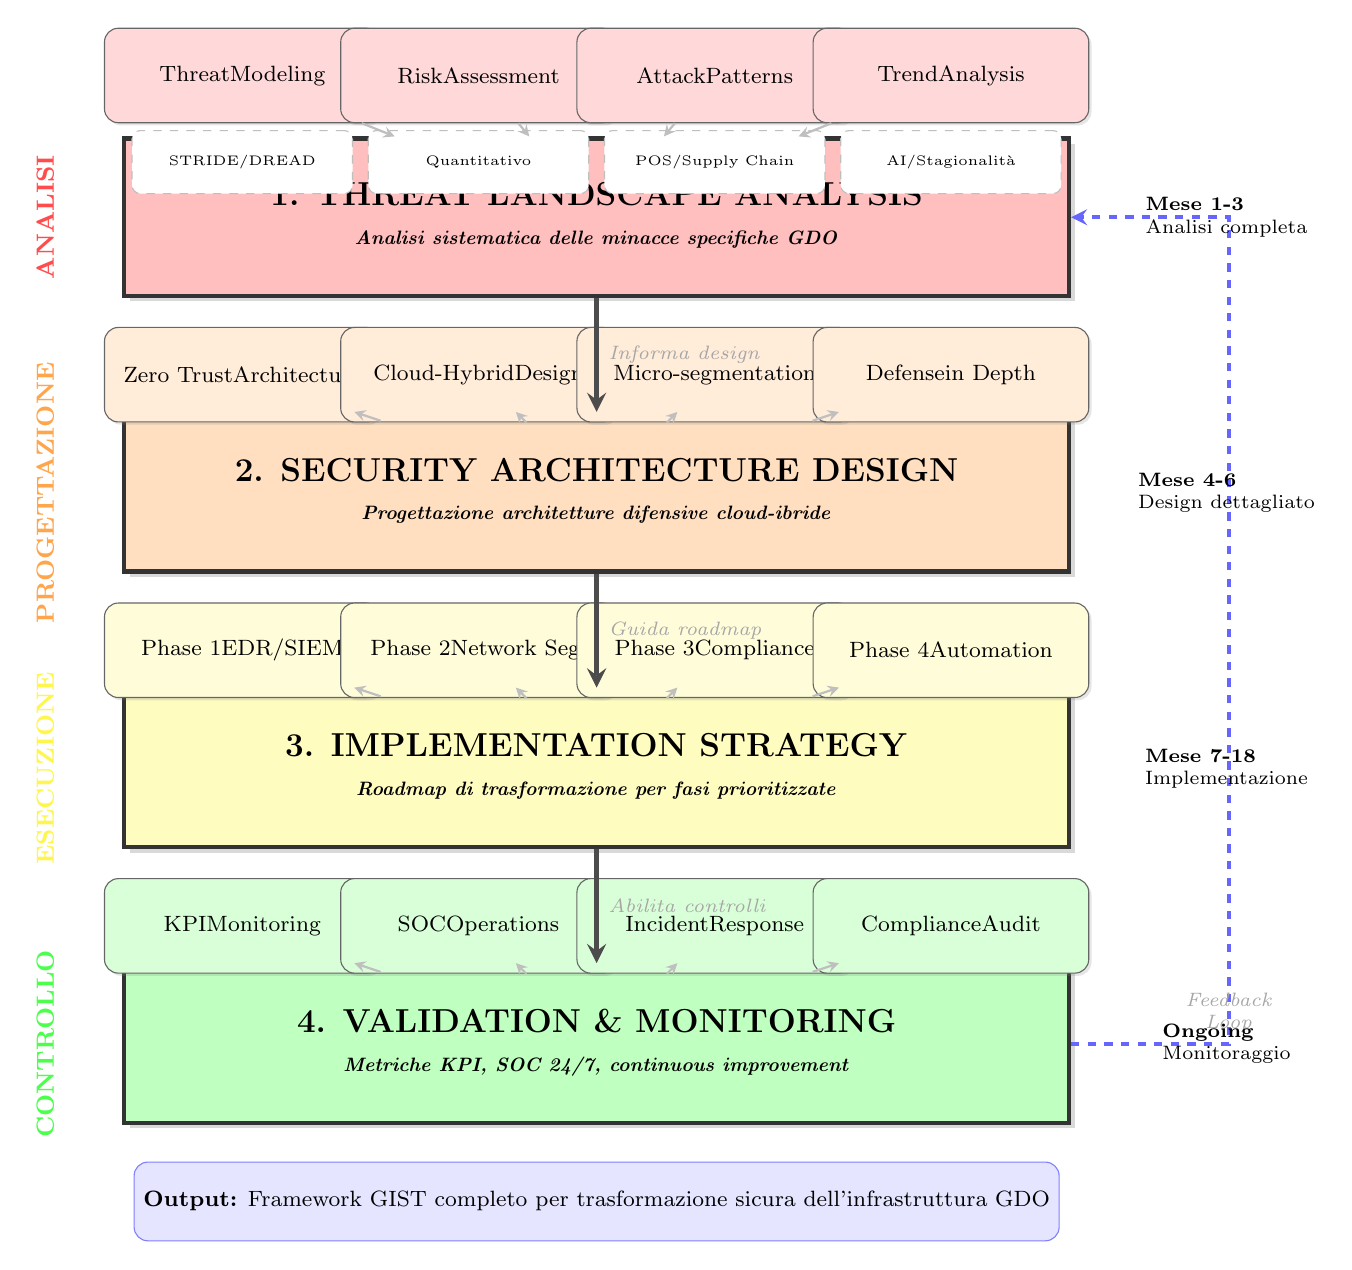
\begin{tikzpicture}[
    % Stili per i box principali
    mainbox/.style={
        rectangle, 
        draw=black!80, 
        line width=1.5pt,
        text centered, 
        minimum width=12cm, 
        minimum height=2cm,
        font=\large\bfseries,
        drop shadow={shadow xshift=2pt, shadow yshift=-2pt, opacity=0.3}
    },
    % Stili per i componenti
    component/.style={
        rectangle, 
        draw=black!60,
        rounded corners=5pt,
        text centered, 
        minimum width=3.5cm, 
        minimum height=1.2cm, 
        font=\footnotesize,
        drop shadow={shadow xshift=1pt, shadow yshift=-1pt, opacity=0.2}
    },
    % Stili per le sottofasi
    subphase/.style={
        rectangle,
        draw=gray!50,
        dashed,
        rounded corners=3pt,
        text centered,
        minimum width=2.8cm,
        minimum height=0.8cm,
        font=\scriptsize,
        fill=white
    },
    % Stili per le frecce
    arrow/.style={->, thick, >=stealth, color=black!70},
    feedback/.style={->, thick, >=stealth, color=blue!60, dashed},
    % Stili per le etichette
    label/.style={font=\scriptsize\itshape, text=gray!70}
]

% LIVELLO 1: Threat Landscape Analysis
\node[mainbox, fill=red!25] (threat) at (0,0) {
    \begin{tabular}{c}
        \textbf{1. THREAT LANDSCAPE ANALYSIS}\\
        \scriptsize\textit{Analisi sistematica delle minacce specifiche GDO}
    \end{tabular}
};

% Componenti del Threat Landscape
\node[component, fill=red!15] (threat_model) at (-4.5,1.8) {Threat\\Modeling};
\node[component, fill=red!15] (risk_assess) at (-1.5,1.8) {Risk\\Assessment};
\node[component, fill=red!15] (attack_patterns) at (1.5,1.8) {Attack\\Patterns};
\node[component, fill=red!15] (trend_analysis) at (4.5,1.8) {Trend\\Analysis};

% Sottoelementi per ogni componente
\node[subphase] at (-4.5,0.7) {\tiny STRIDE/DREAD};
\node[subphase] at (-1.5,0.7) {\tiny Quantitativo};
\node[subphase] at (1.5,0.7) {\tiny POS/Supply Chain};
\node[subphase] at (4.5,0.7) {\tiny AI/Stagionalità};

% LIVELLO 2: Security Architecture Design
\node[mainbox, fill=orange!25] (architecture) at (0,-3.5) {
    \begin{tabular}{c}
        \textbf{2. SECURITY ARCHITECTURE DESIGN}\\
        \scriptsize\textit{Progettazione architetture difensive cloud-ibride}
    \end{tabular}
};

% Componenti dell'architettura
\node[component, fill=orange!15] (zero_trust) at (-4.5,-2) {Zero Trust\\Architecture};
\node[component, fill=orange!15] (cloud_hybrid) at (-1.5,-2) {Cloud-Hybrid\\Design};
\node[component, fill=orange!15] (microseg) at (1.5,-2) {Micro-\\segmentation};
\node[component, fill=orange!15] (defense) at (4.5,-2) {Defense\\in Depth};

% LIVELLO 3: Implementation Strategy
\node[mainbox, fill=yellow!25] (implementation) at (0,-7) {
    \begin{tabular}{c}
        \textbf{3. IMPLEMENTATION STRATEGY}\\
        \scriptsize\textit{Roadmap di trasformazione per fasi prioritizzate}
    \end{tabular}
};

% Fasi di implementazione
\node[component, fill=yellow!15] (phase1) at (-4.5,-5.5) {Phase 1\\EDR/SIEM};
\node[component, fill=yellow!15] (phase2) at (-1.5,-5.5) {Phase 2\\Network Seg.};
\node[component, fill=yellow!15] (phase3) at (1.5,-5.5) {Phase 3\\Compliance};
\node[component, fill=yellow!15] (phase4) at (4.5,-5.5) {Phase 4\\Automation};

% LIVELLO 4: Validation & Monitoring
\node[mainbox, fill=green!25] (validation) at (0,-10.5) {
    \begin{tabular}{c}
        \textbf{4. VALIDATION \& MONITORING}\\
        \scriptsize\textit{Metriche KPI, SOC 24/7, continuous improvement}
    \end{tabular}
};

% Componenti di validazione
\node[component, fill=green!15] (metrics) at (-4.5,-9) {KPI\\Monitoring};
\node[component, fill=green!15] (soc) at (-1.5,-9) {SOC\\Operations};
\node[component, fill=green!15] (incident) at (1.5,-9) {Incident\\Response};
\node[component, fill=green!15] (audit) at (4.5,-9) {Compliance\\Audit};

% Frecce principali di flusso
\draw[arrow, line width=2pt] (threat) -- node[label, right] {Informa design} (architecture);
\draw[arrow, line width=2pt] (architecture) -- node[label, right] {Guida roadmap} (implementation);
\draw[arrow, line width=2pt] (implementation) -- node[label, right] {Abilita controlli} (validation);

% Feedback loop
\draw[feedback, line width=1.5pt] (validation.east) -- ++(2,0) 
    node[label, above, align=center] {Feedback\\Loop} 
    -- ++(0,10.5) -- (threat.east);

% Connessioni tra componenti (frecce sottili)
\foreach \comp in {threat_model, risk_assess, attack_patterns, trend_analysis} {
    \draw[arrow, gray!50] (\comp) -- (threat);
}
\foreach \comp in {zero_trust, cloud_hybrid, microseg, defense} {
    \draw[arrow, gray!50] (\comp) -- (architecture);
}
\foreach \comp in {phase1, phase2, phase3, phase4} {
    \draw[arrow, gray!50] (\comp) -- (implementation);
}
\foreach \comp in {metrics, soc, incident, audit} {
    \draw[arrow, gray!50] (\comp) -- (validation);
}

% Box informativo
\node[rectangle, draw=blue!50, fill=blue!10, rounded corners=5pt, 
      minimum width=11cm, minimum height=1cm, font=\footnotesize] 
      at (0,-12.5) {
    \textbf{Output:} Framework GIST completo per trasformazione sicura dell'infrastruttura GDO
};

% Indicatori laterali
\node[rotate=90, font=\small\bfseries, color=red!70] at (-7,0) {ANALISI};
\node[rotate=90, font=\small\bfseries, color=orange!70] at (-7,-3.5) {PROGETTAZIONE};
\node[rotate=90, font=\small\bfseries, color=yellow!70] at (-7,-7) {ESECUZIONE};
\node[rotate=90, font=\small\bfseries, color=green!70] at (-7,-10.5) {CONTROLLO};

% Timeline indicativa (a destra)
\node[font=\scriptsize, align=left] at (8,0) {\textbf{Mese 1-3}\\Analisi completa};
\node[font=\scriptsize, align=left] at (8,-3.5) {\textbf{Mese 4-6}\\Design dettagliato};
\node[font=\scriptsize, align=left] at (8,-7) {\textbf{Mese 7-18}\\Implementazione};
\node[font=\scriptsize, align=left] at (8,-10.5) {\textbf{Ongoing}\\Monitoraggio};

\end{tikzpicture}
\end{document}